\cxset{
 name={},
 numbering=arabic,
 number font-size=HUGE,
 number font-family=sffamily,
 number font-weight=bfseries,
 number before={},
 number dot=,
 number position=leftname,
 chapter font-family=sffamily,
 chapter font-weight=normalfont,
 chapter font-size=LARGE,
 number after={},
 chapter before={\vspace*{50pt}},
 chapter after={\par\vskip12pt},
 chapter color= sweet,
 number color=black!90,
 title beforeskip=,
% title afterskip={\vspace{30pt}},
 title margin bottom=30pt,
 chapter title align=left,
 title before=,
 title after=,
 title font-family=sffamily,
 title font-color= black!80,
 title font-weight=bfseries,
 title font-size=huge,
 chapter title width=\textwidth,
 chapter title align=raggedright,
 chapter afterindent=false,
 section numbering = arabic,
 section numbering prefix = \thechapter.,
 section indent=0pt,
 section align=left,
 section font-size=Large}
 
 
\chapter{Introduction to style twenty seven }
\lipsum[3]

\medskip
\begin{figure}[ht]
\centering
\fbox{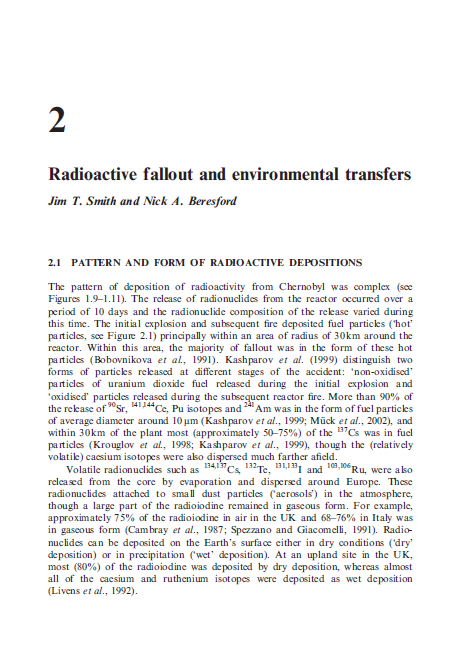
\includegraphics[width=0.5\textwidth]{./chapters/chapter27.png}}
\end{figure}

\section{PATHWAY AND FORM OF RADIOACTIVE DEPOSITIONS}


\lipsum[2-3]

